\section{Implemented code}

Two solutions were implemented one using MPI and one using OpenMP. 

/subsection{MPI implementation}
The MPI solution worked by using the following steps.

\begin{enumerate}
	\item Create the master and n slave processes
	\item Load the psf from ./psf.bmp on the master computer
	\item Send the psf to all the slaves
	\item Get a list of all the images present on the master computer in ./Images/
	\item Send an image from the master to each of the slave processes.
	\item Each of the slaves processes the image using the Richardson-Lucy implemention.
	\item The master retrives the image from the slave and saves it to ./Output/
	\item The master sends the slave a new image
\end{enumerate}

In this implemention all the sending and receiving is done syncronsously with the exception of the retriving of the processed images from the slave. This retriving is made asyncronous so that if one of the slaves finishs faster then one that was started before it there is no delay as it waits for the slave before it to finish and send its image.

In the MPI implementaiton all the sending and receiving of images cannot be parrallized. The number of psfs that require sending also increases with the number of processors that are run. A test was conducted to find the time spent in these different sections by processing 20 1024 by 1024 pixel images  using a 3 by 3 psf.The computer used had a 2.0 GHz dual core proccssor and ran one master and one slave process.

The parrallized section took 386.98 seconds

The serilized section took 4.71 seconds

The total time was 391.69 seconds

Measuring the psf transfer times proved problematic as in the tests it was always less then 1 ms. This meant that even for 1000 process it would add less then 1 second of processing time and so the time increase in the serialized time due to it was ignored.

The above results show that 98.90 percent of the program was parrallizeable and to process all ten million images would require roughly 54400 hours of machine time to complete or 2267 days.

Using armdales law the speed up of the process can be given by
\[
 \frac{1}{(1-P) + \frac{P}{S}}
\]

Where P is the amount of parrallizable code (98.90\% in this case) and S is the number of processors. The amount of time in days to complete the calculation can be shown in Figure~\ref{mpi-time-cores}. As can be obsereved the time for one core is 2267 days, ten cores take 250 days, 20 cores take 137 days, 50 cores take 70 days and 100 cores take 47 days. Beyond this point the speed up from additional cores becomes negligible as the unparralizable sections of code take 25 days to execute. 

\begin{figure}[ht]
	\begin{center}
		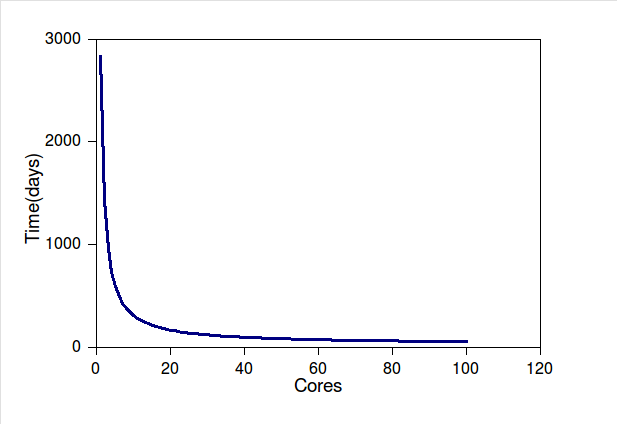
\includegraphics[width=1.0\textwidth]{mpi-time-cores}
	\end{center}
	\caption{Graph showing time to process vs number of cores for the MPI solution}
	\label{mpi-time-cores}
\end{figure}

For running the system the hardware required has to either be rented or brought. A desktop unit with four 3.0 GHz cores costs around \$1000 dollars. For rent the Amazon EC2 service appeared to be the cheapest of the avalibale options charging \$0.68 per hour for use of the High-CPU Extra Large Instance which provideds the following 

\begin{itemize}
\item 7 GB of memory
\item 20 EC2 Compute Units (8 virtual cores with 2.5 EC2 Compute Units each)
\item 1690 GB of instance storage
\item 64-bit platform
\item I/O Performance: High (1 GigaBit ethernet)
\end{itemize}

The EC2 compute units the performance is measured in is equivalent to a 1.0-1.2 GHz 2007 Opteron or 2007 Xeon processor. These processors have roughly 60\% of the processing power of one of the test computers cores. From this information the cost of hiring and buying can be calculated for a set time in which the task has to be completed. This is shown in Figure~\ref{mpi-time-money}. Times below 40 days were not shown as the costs quickly became totally inferable. It can be noted that for processing times longer then 100 days buying units becomes more economical then renting thanks to the one off cost rather then the cost per hour for the cpu time. It should be motioned that the cloud also offers 1 year of use for the much reduced price of \$1820 however at this point a single computer can perform the calculations in 1 year and 15 days and costs only \$1000.

\begin{figure}[ht]
	\begin{center}
		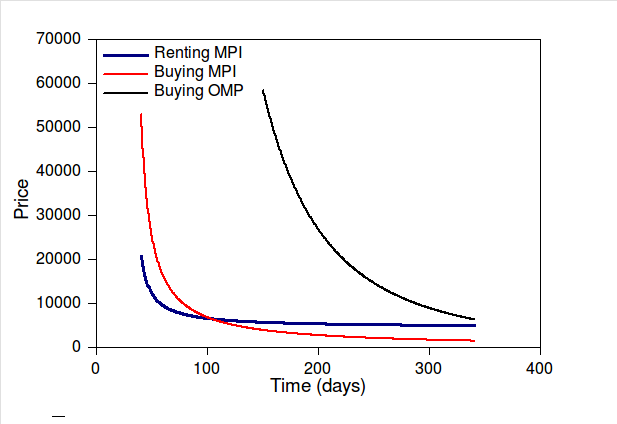
\includegraphics[width=1.0\textwidth]{mpi-time-money}
	\end{center}
	\caption{Cost comparision for the MPI solution taking into account time to complete}
	\label{mpi-time-money}
\end{figure}
